\documentclass[tikz,border=6pt]{standalone}
\usetikzlibrary{arrows.meta,positioning,calc}
\usepackage[T1]{fontenc}
\usepackage{lmodern}
\usepackage{amsmath}

\begin{document}
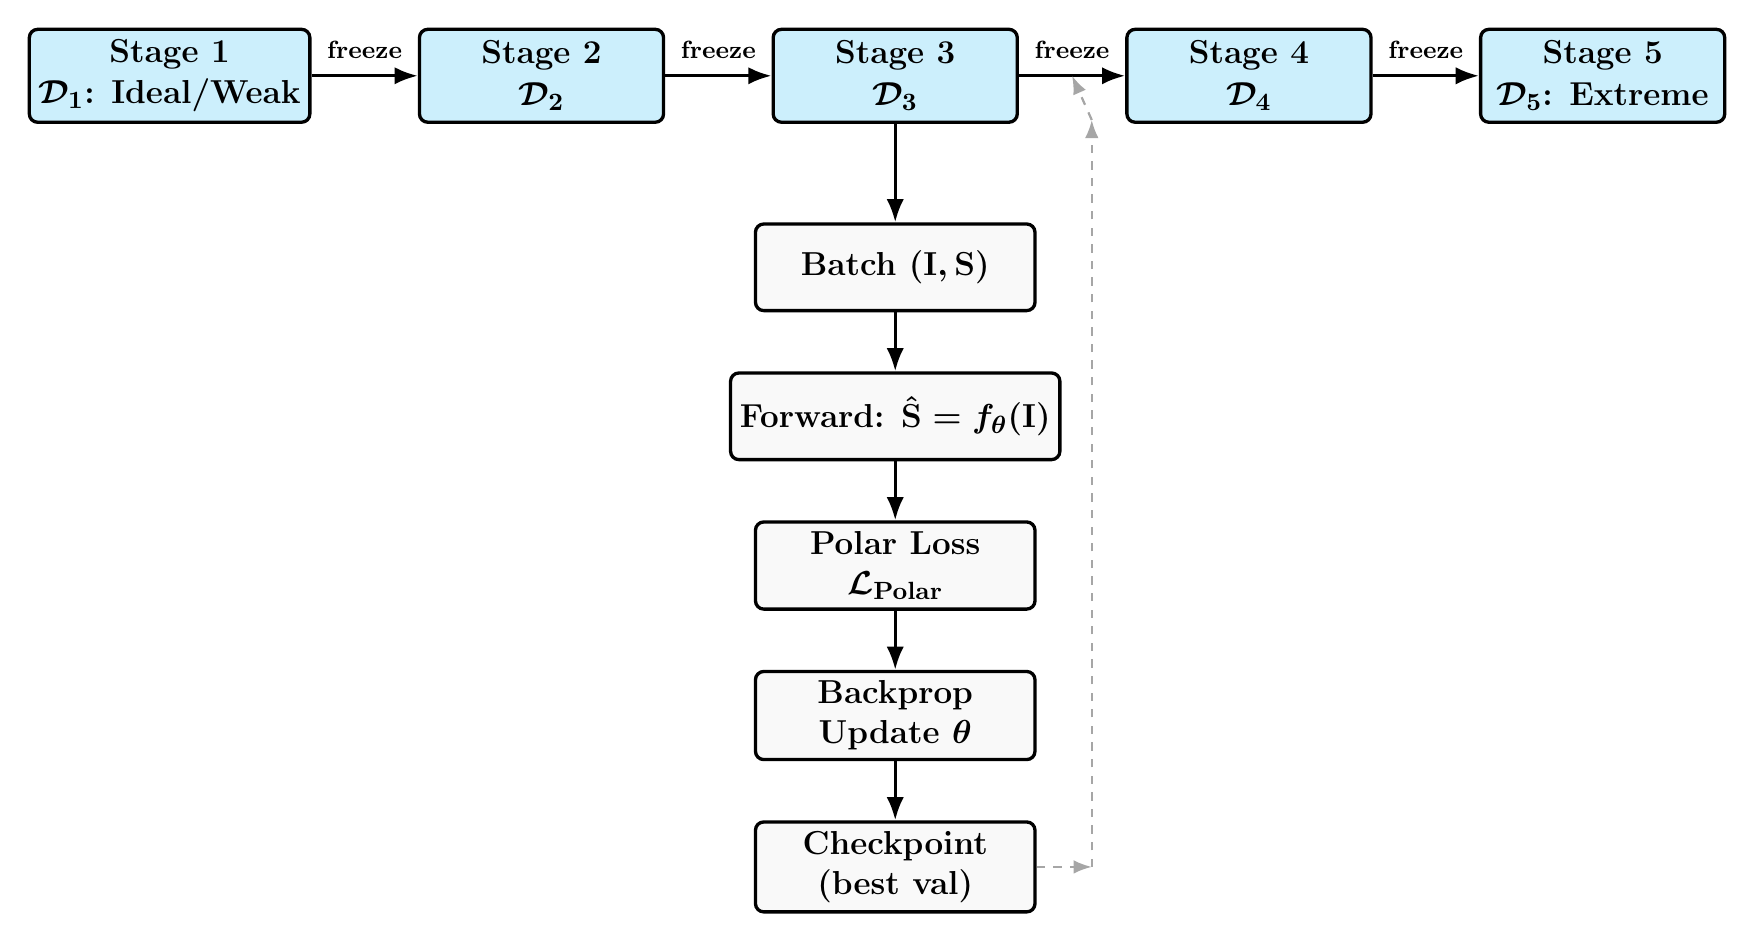
\begin{tikzpicture}[
  >=Latex,
  font=\sffamily,
  flow/.style={-Latex, very thick},
  stage/.style={
    draw, rounded corners=3pt, very thick, align=center,
    minimum width=3.1cm, minimum height=1.18cm, fill=cyan!20,
    font=\bfseries\boldmath\fontsize{13}{15}\selectfont
  },
  proc/.style={
    draw, rounded corners=3pt, very thick, align=center,
    minimum width=3.55cm, minimum height=1.10cm, fill=gray!5,
    font=\bfseries\boldmath\fontsize{12.5}{14.5}\selectfont
  },
  freeze/.style={font=\bfseries\fontsize{9.5}{11}\selectfont},
  dashlink/.style={-Latex, thick, dashed, gray!70}
]

% Top curriculum stages
\node[stage] (s1) {Stage 1\\$\mathcal{D}_1$: Ideal/Weak};
\node[stage, right=1.35cm of s1] (s2) {Stage 2\\$\mathcal{D}_2$};
\node[stage, right=1.35cm of s2] (s3) {Stage 3\\$\mathcal{D}_3$};
\node[stage, right=1.35cm of s3] (s4) {Stage 4\\$\mathcal{D}_4$};
\node[stage, right=1.35cm of s4] (s5) {Stage 5\\$\mathcal{D}_5$: Extreme};

\draw[flow] (s1) -- (s2);
\draw[flow] (s2) -- (s3);
\draw[flow] (s3) -- (s4);
\draw[flow] (s4) -- (s5);

\node[freeze, above=1mm of $(s1.east)!0.5!(s2.west)$] {freeze};
\node[freeze, above=1mm of $(s2.east)!0.5!(s3.west)$] {freeze};
\node[freeze, above=1mm of $(s3.east)!0.5!(s4.west)$] {freeze};
\node[freeze, above=1mm of $(s4.east)!0.5!(s5.west)$] {freeze};

% Vertical training loop below Stage 3
\node[proc, below=1.25cm of s3] (p1) {Batch $(\mathbf{I}, \mathbf{S})$};
\node[proc, below=0.75cm of p1] (p2) {Forward: $\hat{\mathbf{S}} = f_{\theta}(\mathbf{I})$};
\node[proc, below=0.75cm of p2] (p3) {Polar Loss\\$\mathcal{L}_{\mathrm{Polar}}$};
\node[proc, below=0.75cm of p3] (p4) {Backprop\\Update $\theta$};
\node[proc, below=0.75cm of p4] (p5) {Checkpoint\\(best val)};

\draw[flow] (s3.south) -- (p1.north);
\draw[flow] (p1) -- (p2);
\draw[flow] (p2) -- (p3);
\draw[flow] (p3) -- (p4);
\draw[flow] (p4) -- (p5);

% Dashed return loop to stage progression (mirrors original)
\coordinate (retA) at ($(p5.east)+(0.70cm,0)$);
\coordinate (retB) at ($(retA |- s3.south)+(0,0.05cm)$);
\draw[dashlink] (p5.east) -- (retA);
\draw[dashlink] (retA) -- (retB);
\draw[dashlink] (retB) -- ($(s3.east)!0.5!(s4.west)$);

\end{tikzpicture}
\end{document}
